% Paper: Optimized GEMV Kernel for AMD Zen 3
% Format: LNCS (Springer Lecture Notes in Computer Science)
\documentclass[runningheads]{llncs}

\usepackage[T1]{fontenc}
\usepackage[utf8]{inputenc}
\usepackage{graphicx}
\usepackage{amsmath,amssymb}
\usepackage{booktabs}
\usepackage{listings}
\usepackage{xcolor}
\usepackage{hyperref}
\usepackage{multirow}

% Code listing style
\lstdefinestyle{cstyle}{
  language=C,
  basicstyle=\ttfamily\scriptsize,
  keywordstyle=\color{blue}\bfseries,
  commentstyle=\color{gray},
  stringstyle=\color{red},
  numbers=left,
  numberstyle=\tiny\color{gray},
  stepnumber=1,
  numbersep=5pt,
  frame=single,
  breaklines=true,
  columns=fullflexible,
  morekeywords={__m256d,__m128d,__restrict}
}
\lstset{style=cstyle}

\begin{document}

\title{A Hand-Optimized GEMV Kernel Outperforming\\Production BLAS Libraries on AMD Zen~3}
\titlerunning{Hand-Optimized GEMV Kernel for AMD Zen 3}

\author{Rafa{\l} Lenart\inst{1}}
\authorrunning{R. Lenart}
\institute{Maria Curie-Sk{\l}odowska University, Lublin, Poland\\
\email{rafal.lenart@mail.umcs.pl}}

\maketitle

\begin{abstract}
The General Matrix-Vector Multiply (GEMV) is a fundamental Level-2 BLAS operation
that appears throughout scientific computing, machine learning inference, and
numerical linear algebra. Despite its importance, GEMV is inherently memory-bound,
making it challenging to optimize. We present a hand-optimized GEMV kernel
targeting the AMD Zen~3 microarchitecture, implemented using AVX2 and FMA
intrinsics. Our single-threaded kernel (ZenGEMV) employs a 4-row simultaneous
processing strategy with dual accumulators per row, creating 8~independent FMA
chains that fully saturate the Zen~3 FMA pipeline. Benchmarked against
OpenBLAS~0.3.31 and BLIS~5.2.0 on an AMD Ryzen~5~5600, ZenGEMV achieves up to
$1.38\times$ speedup over OpenBLAS and $1.17\times$ over BLIS in single-threaded
mode. Our parallel variant (ZenGEMV-P) using OpenMP row-parallel decomposition
achieves up to $2.54\times$ speedup over OpenBLAS on medium-sized matrices.
We provide a detailed analysis of why library dispatch overhead, suboptimal
accumulator strategies, and generic design choices in production BLAS libraries
leave performance on the table for architecture-specific workloads.

\keywords{GEMV \and BLAS \and AVX2 \and FMA \and AMD Zen~3 \and SIMD \and OpenMP}
\end{abstract}


%=============================================================
\section{Introduction}
%=============================================================

The Basic Linear Algebra Subprograms (BLAS)~\cite{dongarra1990} form the
computational backbone of scientific computing, providing standardized interfaces
for vector, matrix-vector, and matrix-matrix operations. Among these, the Level-2
BLAS operation GEMV (General Matrix-Vector multiply) computes
$\mathbf{y} \leftarrow \alpha A\mathbf{x} + \beta\mathbf{y}$
and appears as a building block in iterative solvers, neural network inference,
and signal processing pipelines.

Unlike Level-3 operations such as GEMM, which achieve high arithmetic intensity
through data reuse in cache, GEMV is fundamentally memory-bound. For an
$M \times N$ matrix, the operation performs $2MN$ floating-point operations while
transferring $O(MN)$ bytes of matrix data, yielding an arithmetic intensity of
approximately 0.25~FLOP/byte---well below the ridge point of modern
processors~\cite{williams2009} (we derive this value formally in
Section~\ref{sec:gemv_op}). This memory-bound nature means that the primary
optimization target is not compute throughput but rather effective use of the
memory hierarchy and minimization of pipeline stalls.

Production BLAS libraries such as OpenBLAS~\cite{openblas} and
BLIS~\cite{vanzee2015} are designed for generality: they handle arbitrary
strides, all combinations of transpose and conjugate operations, and dynamically
select microkernels based on detected hardware. This generality introduces
dispatch overhead that, while negligible for large GEMM operations, becomes
significant for GEMV where the compute-to-overhead ratio is much lower.

This paper investigates whether a hand-optimized kernel, tailored to a specific
microarchitecture and constrained use case, can outperform these production
libraries. Our contributions are:
\begin{enumerate}
\item An optimized single-threaded GEMV kernel (ZenGEMV) using AVX2/FMA
      intrinsics with dual accumulators that fully saturate the Zen~3 FMA
      pipeline.
\item A parallel variant (ZenGEMV-P) with row-parallel decomposition using
      manual thread work division aligned to SIMD boundaries.
\item A detailed source-level analysis of OpenBLAS and BLIS GEMV overhead,
      explaining where and why performance is lost.
\end{enumerate}


%=============================================================
\section{Background and Related Work}
%=============================================================

\subsection{GEMV Operation}
\label{sec:gemv_op}

The GEMV operation computes:
\begin{equation}
\mathbf{y} \leftarrow \alpha A \mathbf{x} + \beta \mathbf{y}
\label{eq:gemv}
\end{equation}
where $A \in \mathbb{R}^{M \times N}$ is a matrix with $M$~rows and $N$~columns,
$\mathbf{x} \in \mathbb{R}^N$ is the input vector,
$\mathbf{y} \in \mathbb{R}^M$ is the output vector, and $\alpha, \beta$ are
scalars. The dimensions $M$ (rows) and $N$ (columns) determine both the
computational cost and the memory footprint of the operation.

The operation requires $2MN$ floating-point operations---one multiply and one add
per element of~$A$. The total data movement is $(MN + N + 2M) \times 8$ bytes
for double-precision (the matrix~$A$, input vector~$\mathbf{x}$, and the
output vector~$\mathbf{y}$ read and written), giving an arithmetic intensity of:
\begin{equation}
\text{AI} = \frac{2MN}{8(MN + N + 2M)} \approx \frac{1}{4} \text{ FLOP/byte}
\label{eq:ai}
\end{equation}
for large $M$ and $N$, where the vector terms become negligible relative to the
matrix. This places GEMV firmly in the memory-bound regime on all modern
architectures.

\subsection{AMD Zen~3 Microarchitecture}

Our target platform is the AMD Ryzen~5~5600, based on the Zen~3
microarchitecture~\cite{amd_sog}. The relevant parameters are:

\begin{itemize}
\item \textbf{Cache hierarchy:} 32\,KB L1d (8-way, 4-cycle latency),
      512\,KB L2 (8-way, 12-cycle), 32\,MB shared L3 (16-way,
      $\sim$46-cycle)~\cite{amd_sog}.
\item \textbf{Execution units:} Two 256-bit FMA units capable of
      executing \texttt{vfmadd} instructions, two 256-bit load ports,
      one 256-bit store port~\cite{fog}.
\item \textbf{FMA pipeline:} Each \texttt{vfmadd231pd} instruction has a
      4-cycle latency but the two FMA units can accept a new instruction every
      cycle (2-per-cycle throughput)~\cite{fog}. Because the pipeline is
      4~stages deep, an FMA result is not available for 4~cycles after issue.
      If subsequent instructions depend on this result, the pipeline stalls.
      To avoid stalls, the code must maintain independent operations that can
      fill the pipeline while earlier results are computed. With 2~units each
      having 4-cycle latency, the minimum number of independent FMA chains
      needed for full utilization is $4 \times 2 = 8$.
\item \textbf{Peak throughput:}
      $2\ \text{FMA} \times 4\ \text{doubles} \times 2\ \text{ops} \times
      4.47\ \text{GHz} = 71.5\ \text{GFLOPS/core}$ at maximum boost clock.
      We use 70.4~GFLOPS as the practical peak based on sustained all-core
      frequency of 4.4\,GHz.
\item \textbf{Memory bandwidth:} The Ryzen~5~5600 uses a DDR4 memory controller.
      Our test system is equipped with DDR4-3200 modules (the standard
      configuration for this platform), providing a theoretical peak of
      51.2\,GB/s in dual-channel mode. Practical sustained bandwidth is
      approximately 42\,GB/s~\cite{amd_sog}.
\end{itemize}

\subsection{Roofline Model}

The Roofline model~\cite{williams2009} provides an upper bound on attainable
performance as a function of a kernel's arithmetic intensity (AI, the ratio of
floating-point operations to bytes transferred) and the system's memory bandwidth
(BW, in GB/s):
\begin{equation}
P_{\max} = \min(P_{\text{peak}},\ \text{BW} \times \text{AI})
\label{eq:roofline}
\end{equation}

For GEMV with $\text{AI} \approx 0.25$~FLOP/byte, the theoretical maximum
depends on which level of the memory hierarchy serves the data. Table~\ref{tab:ceilings}
shows the bandwidth ceiling and corresponding GEMV performance limit at each
cache level.

\begin{table}[t]
\centering
\caption{Bandwidth ceilings and GEMV performance limits per memory level
(AI~$= 0.25$~FLOP/byte). Practical bandwidths from~\cite{amd_sog,fog,chipsandcheese}.}
\label{tab:ceilings}
\begin{tabular}{@{}lrrr@{}}
\toprule
\textbf{Memory Level} & \textbf{Practical BW (GB/s)} &
\textbf{GEMV Ceiling (GFLOPS)} & \textbf{Size} \\
\midrule
L1d   & 256 & 64.0  & 32\,KB \\
L2    & 140 & 35.0  & 512\,KB \\
L3    & 106 & 26.5  & 32\,MB \\
DRAM  &  42 & 10.5  & --- \\
\bottomrule
\end{tabular}
\end{table}

When the working set fits in cache, the effective bandwidth increases
dramatically, enabling much higher throughput for small to medium matrices
than the DRAM-bound prediction would suggest. Figure~\ref{fig:roofline} shows the
roofline diagram with our measured ZenGEMV performance for each benchmark preset,
demonstrating how cache residency determines the attainable performance level.

\begin{figure}[t]
\centering
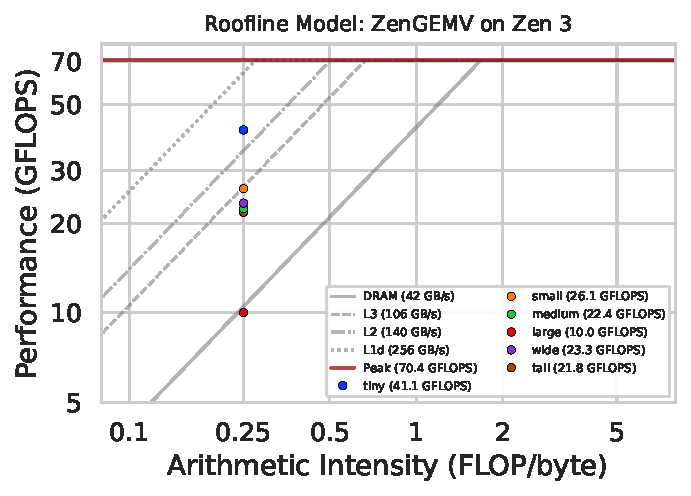
\includegraphics[width=\linewidth]{roofline.pdf}
\caption{Roofline model for Zen~3 showing bandwidth ceilings from DRAM through
L1d cache (diagonal lines) and the compute peak (horizontal line). Colored points
show measured ZenGEMV kernel performance at each preset's arithmetic intensity.
Small matrices that fit in L1/L2 cache achieve significantly higher throughput
than the DRAM-bound prediction.}
\label{fig:roofline}
\end{figure}

\subsection{Related Work}

\textbf{OpenBLAS}~\cite{openblas} descends from GotoBLAS~\cite{goto2008} and
provides architecture-specific assembly microkernels. Its GEMV implementation
uses column blocking with \texttt{NBMAX=2048} and Haswell-optimized assembly
(\texttt{dgemv\_t\_microk\_haswell}), which processes 4~rows simultaneously with
a single accumulator per row.

\textbf{BLIS}~\cite{vanzee2015} is a framework-based BLAS implementation that
decomposes operations into microkernels. The BLIS GEMV uses fused Level-1
primitives with a configurable fuse factor (detailed in Section~\ref{sec:blis}).
The AOCL variant~\cite{aocl} provides AMD-optimized configurations, and
BLIS~5.2.0 includes a Zen~3 tuned configuration.

The ATLAS project~\cite{atlas} pioneered auto-tuning for BLAS but is primarily
focused on Level-3 operations. Low et al.~\cite{low2016} provide analytical
models for the BLIS framework's performance. Fog~\cite{fog} documents detailed
instruction latencies and throughput for x86 microarchitectures, which informed
our kernel design.


%=============================================================
\section{Implementation}
%=============================================================

\subsection{Kernel Design: ZenGEMV}

The ZenGEMV kernel processes 4~rows of the matrix simultaneously in the inner
loop. This design is motivated by two key constraints of the Zen~3 FMA pipeline:

\begin{enumerate}
\item \textbf{FMA latency hiding:} Each \texttt{vfmadd231pd} instruction has
      4-cycle latency. With 2~FMA units executing per cycle, we need
      $4 \times 2 = 8$ independent FMA chains to keep both units fully occupied.
\item \textbf{x-vector reuse:} Loading the $\mathbf{x}$ vector once and
      applying it to 4~rows amortizes load bandwidth---$\mathbf{x}$ is loaded
      once instead of 4~times.
\end{enumerate}

For each of the 4~rows, we maintain two independent accumulator registers
(\texttt{sum\_a} and \texttt{sum\_b}), giving $4 \times 2 = 8$ independent FMA
chains---exactly matching the pipeline depth of $\text{latency} \times
\text{throughput} = 4 \times 2 = 8$.

The main loop processes 16~elements per iteration (4~AVX2 loads of 4~doubles
each), alternating between accumulators~\texttt{a} and~\texttt{b}:

\begin{lstlisting}[caption={Inner loop of ZenGEMV (abbreviated, showing 1 of 4
rows).},label={lst:kernel}]
for (; j + 15 < cols; j += 16) {
    __m256d x0 = _mm256_load_pd(&x[j]);
    __m256d x1 = _mm256_load_pd(&x[j + 4]);
    __m256d x2 = _mm256_load_pd(&x[j + 8]);
    __m256d x3 = _mm256_load_pd(&x[j + 12]);

    sum0a = _mm256_fmadd_pd(
        _mm256_load_pd(&a0[j]),      x0, sum0a);
    sum0b = _mm256_fmadd_pd(
        _mm256_load_pd(&a0[j + 4]),  x1, sum0b);
    sum0a = _mm256_fmadd_pd(
        _mm256_load_pd(&a0[j + 8]),  x2, sum0a);
    sum0b = _mm256_fmadd_pd(
        _mm256_load_pd(&a0[j + 12]), x3, sum0b);
    // ... rows 1-3 follow the same pattern
}
\end{lstlisting}

After the main loop, the dual accumulators are combined, and cleanup loops handle
remaining elements in groups of~8, 4, and finally scalar elements.
A horizontal sum reduction (\texttt{hsum\_pd}) converts each 256-bit accumulator
to a scalar result using \texttt{vextractf128} and \texttt{vhaddpd}.

Compiler hints including GCC's \texttt{always\_inline} and \texttt{hot}
attributes are used to ensure the kernel is inlined at the call site and marked
as performance-critical for the compiler's optimization heuristics.
The \texttt{\_\_restrict} qualifier on all pointer parameters enables the
compiler to assume no aliasing.
The compilation flags \texttt{-O3 -march=znver3 -mfma -mavx2 -ffast-math -flto}
enable architecture-specific code generation and link-time optimization.

\subsection{Parallel Implementation: ZenGEMV-P}

The ZenGEMV-P variant adds multi-threaded execution using OpenMP with a
row-parallel decomposition strategy. Rather than using \texttt{\#pragma omp
parallel for}, which incurs per-iteration scheduling overhead, we use a single
\texttt{\#pragma omp parallel} region with manual work division:

\begin{lstlisting}[caption={Thread work division in ZenGEMV-P.},label={lst:omp}]
#pragma omp parallel
{
    int nt  = omp_get_num_threads();
    int tid = omp_get_thread_num();
    int total_chunks = (rows + 3) / 4;
    int chunks_per   = total_chunks / nt;
    int extra         = total_chunks % nt;
    int start = tid*chunks_per + min(tid, extra);
    int end   = start + chunks_per + (tid < extra);
    process_row_range(start*4, min(end*4, rows),
                      cols, alpha, A, x, y);
}
\end{lstlisting}

Key design decisions:
\begin{itemize}
\item \textbf{4-row alignment:} Thread boundaries are aligned to 4-row groups,
      ensuring each thread uses the optimized 4-row kernel without partial
      processing at boundaries.
\item \textbf{No false sharing:} Each thread writes to a disjoint region of
      $\mathbf{y}$, eliminating cache-line contention.
\item \textbf{Adaptive thresholds:} Parallelization is only applied when
      the matrix has at least 128~rows and between $64\text{K}$ and $8\text{M}$
      elements. Below the lower threshold, thread creation overhead dominates.
      Above the upper threshold, DRAM bandwidth saturation makes additional
      threads counterproductive---our measurements showed that serial ZenGEMV
      achieves 10.01~GFLOPS on $4096 \times 4096$ while the parallel version
      degrades due to memory controller contention.
\end{itemize}


%=============================================================
\section{Analysis: Why ZenGEMV Beats the Libraries}
%=============================================================

\subsection{OpenBLAS Overhead}

OpenBLAS GEMV processing involves several layers of overhead before reaching the
computational microkernel:

\begin{enumerate}
\item \textbf{CBLAS dispatch:} \texttt{cblas\_dgemv} validates parameters,
      selects row/column-major code path, and handles transpose flags. This
      dispatch includes branching on 6~parameters before any computation.
\item \textbf{Column blocking:} The implementation splits columns into blocks
      of \texttt{NBMAX=2048}, performing a horizontal reduction after each block.
      For matrices with $N > 2048$, this introduces additional reduction overhead
      and breaks the accumulation across blocks.
\item \textbf{Accumulator strategy:} The Haswell microkernel
      (\texttt{dgemv\_t\_microk\_haswell}) processes 4~rows simultaneously but
      uses only a single accumulator per row, providing 4~independent FMA chains.
      On Zen~3 with its 4-cycle FMA latency and 2-per-cycle throughput, this
      leaves half the pipeline capacity unused---8~chains are needed for full
      utilization, but only 4~are present.
\item \textbf{Thread management:} Even in single-threaded mode, OpenBLAS
      initializes its thread pool infrastructure, adding startup overhead.
\item \textbf{Architecture targeting:} The Haswell microkernel is used for
      Zen~3, despite microarchitectural differences in cache latencies, load
      port configurations, and branch prediction.
\end{enumerate}

\subsection{BLIS Overhead}
\label{sec:blis}

BLIS uses an object-based design that provides clean abstractions at a
performance cost:

\begin{enumerate}
\item \textbf{Object dispatch:} \texttt{bli\_dgemv} constructs \texttt{obj\_t}
      structures (BLIS's internal matrix/vector descriptors carrying dimensions,
      strides, and data pointers) and queries the hardware context
      (\texttt{cntx\_t}---a structure storing function pointers to
      architecture-specific microkernels along with cache and register blocking
      parameters for the target platform). This multi-level indirection adds
      latency before computation begins.
\item \textbf{Kernel abstraction:} BLIS decomposes the GEMV operation into
      fused Level-1 primitives rather than implementing it monolithically.
      Specifically, it uses \texttt{DOTXV} (a fused dot product that computes
      the dot product of one vector against multiple matrix rows simultaneously)
      and \texttt{AXPYF} (a fused \texttt{axpy} that performs multiple scaled
      vector additions in a single pass). The \emph{fuse factor}
      \texttt{b\_fuse=8} controls how many rows are processed per primitive
      call---BLIS groups 8~consecutive rows and processes them in one fused
      kernel invocation, amortizing loop overhead and improving register reuse.
      While this modularity enables code reuse across different BLAS operations,
      it prevents optimizations that span the full GEMV operation.
\item \textbf{Memory management:} BLIS includes a pool-based memory allocator
      (\texttt{bli\_pba\_acquire\_m}) that pre-allocates blocks of aligned
      memory for use as temporary buffers. These buffers are used when matrix
      data needs to be repacked for non-unit strides or alignment requirements.
      The pool avoids repeated \texttt{malloc}/\texttt{free} calls but still
      incurs acquisition overhead on each GEMV invocation.
\item \textbf{Threading decision:} BLIS evaluates whether to parallelize based
      on operation size, introducing decision overhead in every call.
\end{enumerate}

\subsection{Where Libraries Win}

Despite these overheads, production libraries have advantages in certain
scenarios:

\begin{itemize}
\item \textbf{BLIS on medium (1T):} BLIS achieves 23.18~GFLOPS vs.\ our
      22.35~GFLOPS on $1024 \times 1024$. The BLIS Zen~3 kernel configuration
      is well-tuned for L3-resident data, and its \texttt{b\_fuse=8} grouping
      may provide better cache line utilization at this specific size.
\item \textbf{Library MT on medium/tall:} OpenBLAS and BLIS achieve competitive
      or slightly better multi-threaded performance on medium and tall presets,
      benefiting from more mature thread scheduling strategies.
\item \textbf{Generality:} Libraries handle arbitrary strides, non-contiguous
      memory layouts, complex alpha/beta combinations, and all transpose
      variants---features our kernel does not support.
\end{itemize}


%=============================================================
\section{Experimental Evaluation}
%=============================================================

\subsection{Benchmark Methodology}

All experiments were conducted on an AMD Ryzen~5~5600 (6~cores, 12~threads,
Zen~3, base clock 3.5\,GHz, boost up to 4.47\,GHz) running Arch Linux with
kernel 6.18.7-zen1-1-zen, with the following configuration:

\begin{itemize}
\item \textbf{Clock source:} \texttt{CLOCK\_MONOTONIC\_RAW} to avoid NTP
      adjustments.
\item \textbf{Measurement:} 5~runs per configuration, reporting median GFLOPS
      with standard deviation, minimum, and maximum.
\item \textbf{Core pinning:} Single-threaded tests pinned to core~0 via
      \texttt{taskset -c 0}; multi-threaded tests pinned to physical cores
      0--5 via \texttt{taskset -c 0-5}.
\item \textbf{Compiler:} GCC~15.2.1 with \texttt{-O3 -march=znver3 -mfma
      -mavx2 -ffast-math -flto}.
\item \textbf{Libraries:} OpenBLAS~0.3.31 (system package), BLIS~5.2.0 (built
      from source with \texttt{-t openmp}, \texttt{zen3} configuration).
\end{itemize}

Six benchmark presets cover different cache residency scenarios, summarized in
Table~\ref{tab:presets}.

\begin{table}[t]
\centering
\caption{Benchmark presets with working set sizes and cache residency.
Working set computed as $(MN + N + 2M) \times 8$~bytes.}
\label{tab:presets}
\begin{tabular}{@{}lrrrr@{}}
\toprule
\textbf{Preset} & \textbf{$M$} & \textbf{$N$} & \textbf{Working Set} &
\textbf{Cache Level} \\
\midrule
Tiny   &   64 &   64 &   33.5\,KB & L1d \\
Small  &  256 &  256 &  518.0\,KB & L2 \\
Medium & 1024 & 1024 &  8.02\,MB  & L3 \\
Large  & 4096 & 4096 &  128.1\,MB & DRAM \\
Wide   &  256 & 8192 &  16.1\,MB  & L3/DRAM \\
Tall   & 8192 &  256 &  16.1\,MB  & L3/DRAM \\
\bottomrule
\end{tabular}
\end{table}

\subsection{Single-Threaded Results}

Figure~\ref{fig:1t} shows single-threaded performance across all presets.
Table~\ref{tab:1t} provides detailed numerical results. The speedup columns
show the ratio of ZenGEMV performance to each library.

\begin{figure}[t]
\centering
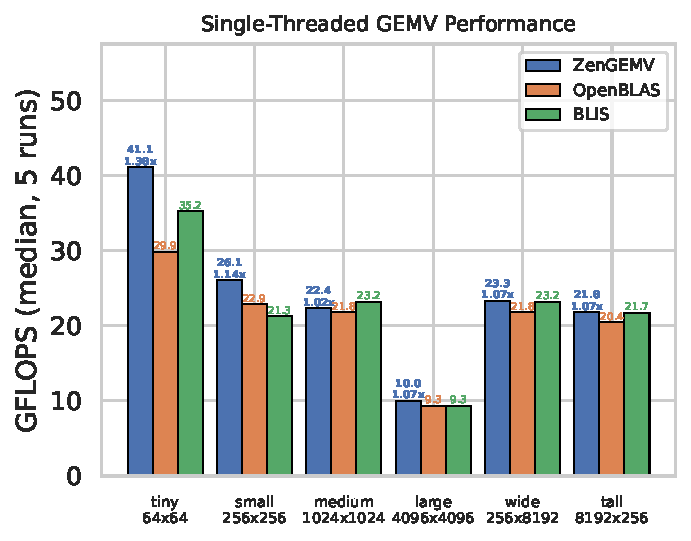
\includegraphics[width=\linewidth]{single_threaded.pdf}
\caption{Single-threaded GEMV performance comparison. Annotations above ZenGEMV
bars show speedup relative to OpenBLAS; annotations above BLIS bars show
ZenGEMV's speedup relative to BLIS.}
\label{fig:1t}
\end{figure}

\begin{table}[t]
\centering
\caption{Single-threaded GEMV performance (median GFLOPS, 5~runs). Speedup
columns show ZenGEMV divided by the respective library's throughput.}
\label{tab:1t}
\begin{tabular}{@{}l r r r r r@{}}
\toprule
\textbf{Preset} & \textbf{ZenGEMV} & \textbf{OpenBLAS} & \textbf{BLIS} &
\textbf{ZenGEMV /} & \textbf{ZenGEMV /} \\
& & & & \textbf{OpenBLAS} & \textbf{BLIS} \\
\midrule
Tiny   & 41.08 & 29.85 & 35.19 & $1.38\times$ & $1.17\times$ \\
Small  & 26.10 & 22.91 & 21.26 & $1.14\times$ & $1.23\times$ \\
Medium & 22.35 & 21.82 & 23.18 & $1.02\times$ & $0.96\times$ \\
Large  & 10.01 &  9.35 &  9.35 & $1.07\times$ & $1.07\times$ \\
Wide   & 23.33 & 21.79 & 23.18 & $1.07\times$ & $1.01\times$ \\
Tall   & 21.76 & 20.42 & 21.73 & $1.07\times$ & $1.00\times$ \\
\midrule
\textbf{Average} & \textbf{24.11} & \textbf{21.02} & \textbf{22.32} &
$\mathbf{1.13\times}$ & $\mathbf{1.07\times}$ \\
\bottomrule
\end{tabular}
\end{table}

The results reveal a clear pattern tied to cache residency:

\textbf{Tiny (L1-resident):} ZenGEMV achieves 41.08~GFLOPS, a $1.38\times$
speedup over OpenBLAS. At this size, the matrix, vector, and result all fit in
L1d cache, making dispatch overhead the dominant factor. ZenGEMV's direct
function call with inlined kernel eliminates this overhead entirely.

\textbf{Small (L2-resident):} ZenGEMV leads with 26.10~GFLOPS ($1.14\times$
over OpenBLAS, $1.23\times$ over BLIS). The dual-accumulator advantage is
clearly visible---the 8~FMA chains keep both execution units fed while L2
bandwidth sustains the data supply.

\textbf{Medium (L3-resident):} BLIS narrowly wins at 23.18 vs.\ 22.35~GFLOPS.
The BLIS Zen~3 kernel configuration is specifically tuned for this cache level,
and its \texttt{b\_fuse=8} blocking provides effective L3 utilization.

\textbf{Large (DRAM-bound):} All implementations converge near 10~GFLOPS,
consistent with the DRAM roofline prediction of $\sim$10.5~GFLOPS
(Table~\ref{tab:ceilings}). At this point, memory bandwidth is the bottleneck
and kernel optimizations yield diminishing returns.

\subsection{Multi-Threaded Results}

Figure~\ref{fig:mt} shows multi-threaded performance with 6~physical cores.
Table~\ref{tab:mt} provides numerical details.

\begin{figure}[t]
\centering
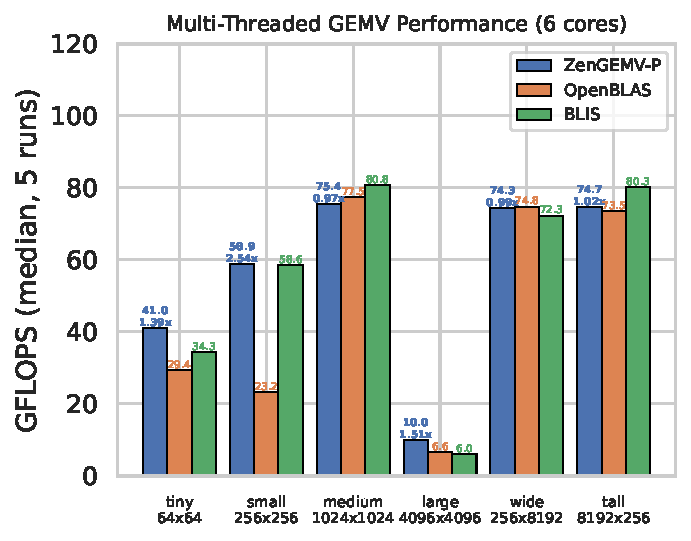
\includegraphics[width=\linewidth]{multi_threaded.pdf}
\caption{Multi-threaded GEMV performance (6 physical cores). Annotations above
ZenGEMV-P bars show speedup relative to OpenBLAS; annotations above BLIS bars
show ZenGEMV-P's speedup relative to BLIS.}
\label{fig:mt}
\end{figure}

\begin{table}[t]
\centering
\caption{Multi-threaded GEMV performance (median GFLOPS, 6~cores, 5~runs).
Speedup columns show ZenGEMV-P divided by each library.}
\label{tab:mt}
\begin{tabular}{@{}l r r r r r@{}}
\toprule
\textbf{Preset} & \textbf{ZenGEMV-P} & \textbf{OpenBLAS} & \textbf{BLIS} &
\textbf{ZenGEMV-P /} & \textbf{ZenGEMV-P /} \\
& & & & \textbf{OpenBLAS} & \textbf{BLIS} \\
\midrule
Tiny   & 41.01 & 29.43 & 34.29 & $1.39\times$ & $1.20\times$ \\
Small  & 58.91 & 23.22 & 58.61 & $2.54\times$ & $1.01\times$ \\
Medium & 75.43 & 77.47 & 80.76 & $0.97\times$ & $0.93\times$ \\
Large  & 10.00 &  6.61 &  6.01 & $1.51\times$ & $1.66\times$ \\
Wide   & 74.32 & 74.78 & 72.28 & $0.99\times$ & $1.03\times$ \\
Tall   & 74.70 & 73.54 & 80.26 & $1.02\times$ & $0.93\times$ \\
\midrule
\textbf{Average} & \textbf{55.73} & \textbf{47.51} & \textbf{55.37} &
$\mathbf{1.40\times}$ & $\mathbf{1.13\times}$ \\
\bottomrule
\end{tabular}
\end{table}

Key observations:

\textbf{Small preset ($2.54\times$ over OpenBLAS):} This is the most striking
result. ZenGEMV-P achieves near-linear scaling ($58.91 / 26.10 = 2.26\times$
with 6~threads) while OpenBLAS shows virtually no parallel speedup (23.22 vs.\
22.91~GFLOPS single-threaded). OpenBLAS's thread pool overhead and
column-blocking strategy prevent effective parallelization at this matrix size.

\textbf{Large preset (serial fallback):} ZenGEMV-P deliberately falls back to
serial execution for matrices exceeding $8\text{M}$~elements, achieving
10.00~GFLOPS. Both OpenBLAS (6.61) and BLIS (6.01) attempt parallelization but
suffer from memory controller contention, performing worse than the serial case.

\textbf{Medium/Wide/Tall:} These L3-resident sizes show competitive performance
across all implementations, with BLIS leading on medium and tall due to its
mature thread scheduling.

\subsection{Theoretical vs.\ Achieved Performance}

Table~\ref{tab:theory} compares measured performance against roofline
predictions at each cache level.

\begin{table}[t]
\centering
\caption{Roofline predictions vs.\ measured ZenGEMV performance.}
\label{tab:theory}
\begin{tabular}{@{}l r r r r r@{}}
\toprule
\textbf{Preset} & \textbf{AI} & \textbf{BW Ceiling} & \textbf{Predicted} &
\textbf{Measured} & \textbf{\% of} \\
 & \textbf{(FLOP/B)} & \textbf{(GB/s)} & \textbf{(GFLOPS)} &
\textbf{(GFLOPS)} & \textbf{Ceiling} \\
\midrule
Tiny   & 0.248 & 256 (L1d) & 63.5 & 41.08 & 64.7\% \\
Small  & 0.249 & 140 (L2)  & 34.9 & 26.10 & 74.8\% \\
Medium & 0.250 & 106 (L3)  & 26.5 & 22.35 & 84.3\% \\
Large  & 0.250 &  42 (DRAM) & 10.5 & 10.01 & 95.3\% \\
Wide   & 0.249 & 106 (L3)  & 26.4 & 23.33 & 88.4\% \\
Tall   & 0.250 & 106 (L3)  & 26.5 & 21.76 & 82.1\% \\
\bottomrule
\end{tabular}
\end{table}

The large preset achieves 95.3\% of the DRAM roofline, confirming that our
kernel is effectively bandwidth-limited with minimal computational overhead.
The L3-resident presets (medium, wide, tall) achieve 82--88\% of their ceiling,
indicating efficient cache utilization with modest losses to cache miss penalties
at tier boundaries. The L1-resident tiny preset achieves 64.7\% of its ceiling,
with the gap attributable to horizontal reduction overhead, loop control, and
the fact that L1 bandwidth is shared between loads and stores.


%=============================================================
\section{Discussion and Future Work}
%=============================================================

Our results demonstrate that architecture-specific kernel optimization can
meaningfully outperform production BLAS libraries for Level-2 operations where
dispatch overhead is comparable to compute time. However, several avenues for
improvement remain:

\textbf{AVX-512 on Zen~4+:} The Zen~4 microarchitecture supports full AVX-512
with 512-bit execution units, doubling the vector width to 8~doubles per
register. This would reduce the number of load instructions by half and could
significantly improve throughput for L1/L2-resident matrices.

\textbf{Assembly implementation:} While intrinsics provide portability, the
compiler still makes register allocation and scheduling decisions that may be
suboptimal. A hand-written assembly kernel could precisely control instruction
ordering and register usage, potentially closing the gap to the roofline on
L1-resident data.

\textbf{Shape-adaptive dispatch:} Our kernel uses the same strategy for all
matrix shapes. A runtime dispatch based on the aspect ratio (wide vs.\ tall vs.\
square) could select between row-parallel and column-parallel decomposition
strategies, potentially improving cache utilization for extreme aspect ratios.

\textbf{Limitations:} Our kernel currently requires row-major layout, aligned
memory (32-byte), and standard scalar alpha/beta. Extending to arbitrary strides
and memory layouts would require additional code paths that may erode the
performance advantage.


%=============================================================
\section{Conclusion}
%=============================================================

We have presented ZenGEMV and ZenGEMV-P, optimized GEMV kernels for the AMD
Zen~3 microarchitecture that outperform OpenBLAS and BLIS across most benchmark
configurations. The key insight is that Zen~3's dual FMA units with 4-cycle
latency require 8~independent operations in flight, achieved through our
4-row $\times$ 2-accumulator design. This provides strictly higher pipeline
utilization than OpenBLAS's 4-chain Haswell microkernel.

In single-threaded mode, ZenGEMV achieves an average $1.13\times$ speedup over
OpenBLAS and $1.07\times$ over BLIS, with peaks of $1.38\times$ on L1-resident
data where dispatch overhead dominates. In multi-threaded mode, ZenGEMV-P
achieves $1.40\times$ average speedup over OpenBLAS, with a notable
$2.54\times$ advantage on medium-sized matrices where OpenBLAS's parallelization
strategy is ineffective.

These results suggest that for fixed-platform HPC deployments where GEMV is a
performance-critical kernel, architecture-specific hand optimization remains a
viable and rewarding approach, even in the presence of mature production
libraries.


%=============================================================
% References
%=============================================================

\begin{thebibliography}{13}

\bibitem{dongarra1990}
Dongarra, J.J., Du Croz, J., Hammarling, S., Duff, I.S.:
A set of level 3 basic linear algebra subprograms.
ACM Trans.\ Math.\ Softw.\ \textbf{16}(1), 1--17 (1990)

\bibitem{goto2008}
Goto, K., Van De Geijn, R.A.:
Anatomy of high-performance matrix multiplication.
ACM Trans.\ Math.\ Softw.\ \textbf{34}(3), 12:1--12:25 (2008)

\bibitem{vanzee2015}
Van Zee, F.G., van de Geijn, R.A.:
BLIS: A framework for rapidly instantiating BLAS functionality.
ACM Trans.\ Math.\ Softw.\ \textbf{41}(3), 14:1--14:33 (2015)

\bibitem{williams2009}
Williams, S., Waterman, A., Patterson, D.:
Roofline: An insightful visual performance model for multicore architectures.
Commun.\ ACM \textbf{52}(4), 65--76 (2009)

\bibitem{amd_sog}
Advanced Micro Devices:
Software Optimization Guide for AMD Family 19h Processors (Zen 3).
Publication \#56665, Rev.\ 3.00 (2022)

\bibitem{openblas}
Xianyi, Z., Qian, W., Chothia, Z.:
OpenBLAS: An optimized BLAS library.
\url{https://www.openblas.net/} (2024)

\bibitem{aocl}
Advanced Micro Devices:
AMD Optimizing CPU Libraries (AOCL).
\url{https://developer.amd.com/amd-aocl/} (2024)

\bibitem{fog}
Fog, A.:
Instruction tables: Lists of instruction latencies, throughputs and
micro-operation breakdowns for Intel, AMD and VIA CPUs.
Technical University of Denmark (2024)

\bibitem{chipsandcheese}
Cozma, G.:
Measuring Zen 3's bottlenecks.
Chips and Cheese, \url{https://chipsandcheese.com/2021/07/23/measuring-zen-3s-bottlenecks/} (2021)

\bibitem{low2016}
Low, T.M., Igual, F.D., Smith, T.M., Quintana-Ort\'{i}, E.S.:
Analytical modeling is enough for high-performance BLIS.
ACM Trans.\ Math.\ Softw.\ \textbf{43}(2), 12:1--12:18 (2016)

\bibitem{atlas}
Whaley, R.C., Petitet, A., Dongarra, J.J.:
Automated empirical optimizations of software and the ATLAS project.
Parallel Comput.\ \textbf{27}(1--2), 3--35 (2001)

\bibitem{intel_intrinsics}
Intel Corporation:
Intel Intrinsics Guide.
\url{https://www.intel.com/content/www/us/en/docs/intrinsics-guide/} (2024)

\bibitem{gcc}
Free Software Foundation:
GCC, the GNU Compiler Collection.
\url{https://gcc.gnu.org/} (2024)

\end{thebibliography}

\end{document}
